% ==================== CHAPTER 3 ====================
\chapter{METHODOLOGY AND SYSTEM ARCHITECTURE}
\clearpage

\section{The Full-Stack Architecture Design}
The system is divided into two major components: Backend \& AI Infrastructure and Client-Side Interfaces, all containerized using Docker for consistent deployment.
\begin{itemize}
    \item \textbf{Backend API (Gin/Go):} Chosen over traditional Python frameworks (like Flask) because Go natively handles thousands of simultaneous feed requests efficiently, matching the high-concurrency needs of social media.
    \item \textbf{Recommendation Engine (Gorse):} Functions as the AutoML core. Gorse automatically optimizes algorithm selection as user density increases. It leverages Redis to cache intermediate results and trending posts (popularity-based recommendations via caching).
    \item \textbf{Frontend Monorepo:} Next.js was utilized with Server Components for web latency optimization and SEO, alongside React Native for mobile. The UI is built using Shadcn UI, Tailwind CSS, and Lucide React. Data validation is enforced via Zod.
\end{itemize}

\section{Algorithm Selection and Integration}

\begin{figure}[htbp]
    \centering
    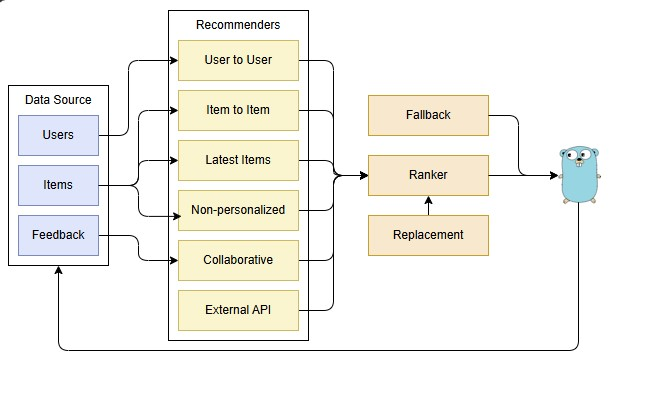
\includegraphics[width=0.9\textwidth]{../media/figers/gorse_architecture.jpg}
    \caption{Architectural Overview of the Gorse Recommendation Engine.}
    \label{fig:gorse-architecture}
\end{figure}

\begin{figure}[htbp]
    \centering
    \resizebox{\textwidth}{!}{\input{../media/figers/gorse_data_flow.tex}}
    \caption{Detailed Data Flow and Request Lifecycle within the Gorse Cluster.}
    \label{fig:gorse-data-flow}
\end{figure}

Instead of manual architecture and hyperparameter tuning, the implementation leverages the AutoML capabilities of Gorse to evaluate and deploy the most effective algorithms dynamically. The recommendation pipeline is decoupled into distinct stages:

\subsection{Core ML Algorithms}
Once candidates are generated, the scoring stage refines the ranking using heavy predictive algorithms.
\begin{itemize}
    \item \textbf{Factorization Machines (FM):} Serving as the core classical ranker within Gorse, FM models interactions between sparse features (e.g., user demographics + post tags) to predict Click-Through Rates (CTR). Mathematically, the degree-2 FM model evaluates the predicted score $\hat{y}$ for a feature vector $\mathbf{x}$ as:
    \begin{equation}
    \hat{y}(\mathbf{x}) = w_0 + \sum_{i=1}^{n} w_i x_i + \sum_{i=1}^{n} \sum_{j=i+1}^{n} \langle \mathbf{v}_i, \mathbf{v}_j \rangle x_i x_j
    \end{equation}
    where $w_0$ is the global bias, $w_i$ models the strength of the $i$-th variable, and $\langle \mathbf{v}_i, \mathbf{v}_j \rangle$ is the dot product of two latent vectors representing the interaction between features $i$ and $j$.
    
    \item \textbf{Bayesian Personalized Ranking (BPR):} Rather than predicting an absolute rating value (Pointwise Mean Squared Error), BPR employs a pairwise loss function that evaluates the probability of a user preferring \textit{Item A} over \textit{Item B}. This is highly optimal for modeling implicit feedback. The BPR optimization criterion maximizes the posterior probability:
    \begin{equation}
    \text{BPR-OPT} = \sum_{(u,i,j) \in D_S} \ln \sigma(\hat{x}_{uij}) - \lambda_\Theta \|\Theta\|^2
    \end{equation}
    where $\hat{x}_{uij} = \hat{y}_{ui} - \hat{y}_{uj}$ denotes the predicted preference of user $u$ for item $i$ over item $j$, $\sigma(\cdot)$ is the logistic sigmoid function, and $\lambda_\Theta$ is a regularization parameter to prevent overfitting.
\end{itemize}

\begin{table}[htbp]
\centering
\caption{The Core ML Algorithms: Factorization Machines vs.\ Industry Alternatives}
\label{tab:core-ml}
\begin{tabularx}{\textwidth}{XXXX}
\toprule
\textbf{\textit{Algorithm Category}} & \textbf{\textit{Implemented Approach}} & \textbf{\textit{Purpose}} & \textbf{\textit{Alternative Considerations}} \\
\midrule
\textbf{\textit{Ranking / Scoring}} & Factorization Machines (FM) & High-precision CTR prediction on sparse data. & DeepFM (Adds Neural Networks for non-linear logic). \\
\rowcolor{gray!10}
\textbf{\textit{Loss Optimization}} & BPR (Pairwise Ranking) & Optimizes sequential item preference ranking. & Pointwise MSE or Listwise optimization. \\
\textbf{\textit{Latent Modeling}} & Matrix Factorization (MF) & Extracts implicit patterns via latent factors. & SVD++ (incorporates implicit feedback dynamically). \\
\bottomrule
\end{tabularx}
\end{table}

\subsection{Candidate Generation}
Because computing FM scores across millions of posts is computationally expensive, candidate generation acts as an initial filtration phase to isolate the top pool.
\begin{itemize}
    \item \textbf{Vector Search (ANN):} Typesense is utilized, powered by the Hierarchical Navigable Small World (HNSW) algorithm. This converts social text into vectors and finds nearest neighbors in sub-milliseconds.
    \item \textbf{Collaborative Filtering \& Popularity:} Gorse implicitly tracks Item-to-Item and User-to-User similarity, utilizing Redis to cache trending global content.
\end{itemize}

\begin{table}[htbp]
\centering
\caption{Candidate Generation (Filter) Techniques and Implementation}
\label{tab:candidate-gen}
\begin{tabularx}{\textwidth}{XXXX}
\toprule
\textbf{\textit{Technique}} & \textbf{\textit{Proposed Implementation}} & \textbf{\textit{Speed / Scale}} & \textbf{\textit{Traditional/Industry Alternative}} \\
\midrule
\textbf{\textit{Vector Search (ANN)}} & Typesense (using HNSW) & Sub-50ms (in-RAM) & FAISS (Meta) or Milvus (Cloud) \\
\rowcolor{gray!10}
\textbf{\textit{Matching Engine}} & Gorse AutoML Pipelines & High-Concurrency Engine & Elasticsearch (BM25 Lexical) \\
\bottomrule
\end{tabularx}
\end{table}

\begin{table}[htbp]
\centering
\caption{Collaborative Filtering and Popularity-Based Techniques}
\label{tab:cf-pop}
\begin{tabularx}{\textwidth}{XXXX}
\toprule
\textbf{\textit{Filter Strategy}} & \textbf{\textit{Implementation in Stack}} & \textbf{\textit{Key Advantage}} & \textbf{\textit{Alternatives}} \\
\midrule
\textbf{\textit{Collaborative Filtering}} & Matrix Factorization (MF) & Extracts latent user-item patterns. & LightGCN (Graph Neural Networks). \\
\rowcolor{gray!10}
\textbf{\textit{Trending/Popularity}} & Redis Memory Caching & Avoids cold-start issues for new users. & Thompson Sampling (Bandit strategies). \\
\bottomrule
\end{tabularx}
\end{table}

\section{Data Collection, NLP Context, and Model Training Materials}
To simulate a real-world environment, the system utilizes industry-standard datasets for diverse behavioral dimensions. Understanding the ``context'' of a social media post requires advanced Natural Language Processing.

\begin{table}[htbp]
\centering
\caption{Natural Language Processing (Context) Tooling Selection}
\label{tab:nlp}
\begin{tabularx}{\textwidth}{XXX}
\toprule
\textbf{\textit{NLP Tooling}} & \textbf{\textit{Functionality}} & \textbf{\textit{Modern AI Alternatives}} \\
\midrule
\textbf{\textit{BERT / RoBERTa}} & Converts social media text strings into semantic numerical vectors. & OpenAI Embeddings (High latency and cost overhead). \\
\rowcolor{gray!10}
\textbf{\textit{Sentence-Transformers}} & Standardized embedding framework for localized vector generation. & Llama 3 / Mistral (Utilized for pre-embedding textual summarization). \\
\bottomrule
\end{tabularx}
\end{table}

\begin{itemize}
    \item \textbf{Interaction Data:} The RecSys Challenge 2020 Twitter Dataset \cite{recsys2020}, containing over 200 million public engagements, serves as the training ground for the predictive models. This natively categorizes explicit interactions (e.g., likes, retweets) and implicit interactions.
    \item \textbf{Social Graph Data:} The Stanford SNAP Twitter Network dataset \cite{snap2014} is used to map ego networks and lists, validating the Collaborative Filtering structures.
    \item \textbf{Content Context:} Embeddings correlate with Sentence-Transformers using models fine-tuned from Sentiment140 data \cite{sentiment140}.
\end{itemize}

\section{System Flow and Recommendation Pipeline}
The operational system follows a sophisticated \textbf{Retrieval $\rightarrow$ Ranking $\rightarrow$ Re-ranking} flowchart, structurally dividing the distributed computational overhead into an Offline Training Pipeline and an Online Retrieval Pipeline.

\subsection{Data Ingestion and Telemetry Architecture}
Before execution, the system captures three primary data streams: \textit{Users} (demographics/tags), \textit{Items} (social media posts), and \textit{Feedback}. Following established behavioral telemetry frameworks, feedback is strictly classified into:
\begin{enumerate}
    \item \textbf{Explicit Signals:} Conscious, manual user actions including ``Likes'', ``Retweets'', and explicit application ratings.
    \item \textbf{Implicit Signals:} Passive behavioral telemetry such as session dwell time, scroll pausing, and click-through reads. Capturing implicit data is critical because users rarely explicitly rate content; utilizing implicit telemetry drastically reduces rating matrix sparsity and provides a significantly more authentic reflection of core user preferences.
\end{enumerate}

To distribute this constant ingestion workload efficiently, the architecture is decoupled into specific operational clusters:
\begin{itemize}
    \item \textbf{Master Node:} Manages global state, schedules background training jobs, and hosts the monitoring dashboard.
    \item \textbf{Worker Nodes:} Execute the heavy CPU/GPU computational lifting for matrix math and neighbor searching.
    \item \textbf{Server Nodes:} Intercept live RESTful API requests natively from the Go (Gin) frontend gateway.
    \item \textbf{Data Layer:} Redis manages online metadata mapping, while persistent state syncs with the primary database.
\end{itemize}

\subsection{The Offline Training Pipeline (Latent Factorization)}
Rather than attempting massive mathematical computations reactively, predictive models are compiled asynchronously in the background. This architectural decoupling ensures that real-time API latency remains incredibly stable. Following the methodologies outlined by Aggarwal \cite{aggarwal2016}, this offline pipeline utilizes rigorous Latent Factor Models:
\begin{itemize}
    \item \textbf{Matrix Factorization and Singular Value Decomposition (SVD):} The engine periodically decomposes the highly sparse user-item interaction matrices into lower-dimensional representations (latent factors). By applying SVD principles, the system inherently maps both users and posts into a shared geometric space, automatically unearthing hidden preferences (i.e.\ mathematically predicting that if User A and User B share historical browsing geometries, their latent vectors will intersect).
    \item \textbf{Stochastic Gradient Descent (SGD) and Regularization:} To prevent mathematical over-fitting, the offline pipeline continually optimizes these latent parameters using Stochastic Gradient Descent. Strict regularization terms are continuously applied to the loss functions, ensuring the model generalizes accurately to new, unseen social feed data instead of strictly memorizing past interactions.
    \item \textbf{CTR Prediction (Factorization Machines):} Continually ingesting updated meta-features and the newly stabilized latent factors, the mathematical weights are optimized against interaction density to predict immediate Click-Through Rates.
\end{itemize}

\subsection{The Online Retrieval Pipeline}
Upon a user refreshing their feed, the system executes the real-time funnel sequentially:
\begin{enumerate}
    \item \textbf{Step A: Candidate Retrieval:} To circumvent ranking millions of items simultaneously, candidate funnels isolate a few hundred target items utilizing Typesense nearest-neighbor similarity and Gorse Collaborative Filtering. To directly counter the ``Cold-Start'' problem (anonymous or brand-new users) and the ``Gray Sheep'' anomaly (users with unpredictable, disjointed tastes), globally trending popular items and explicit programmatic association rules are strategically injected during this localized retrieval phase.
    \item \textbf{Step B: Ranking:} The filtered items are processed through the CTR Model, attaching a strict probability float score (0.0 to 1.0) to ascertain exact user preferences.
    \item \textbf{Step C: Re-Ranking:} Before the payload drops efficiently into the RTK Query cache on the Next.js/React Native frontend, strict business logic is applied. This includes removing duplicate/previously-viewed items globally, and natively applying ``Explore vs.\ Exploit''---injecting strategically randomized items to break programmatic filter bubbles and continuously harvest fresh implicit rating signals.
\end{enumerate}
